% Springer LNCS format.
% Requires: llncs.cls and splncs04.bst from the Springer LNCS package:
%   https://www.springer.com/gp/computer-science/lncs/conference-proceedings-guidelines
% Build:
%   pdflatex main_springer && bibtex main_springer &&
%   pdflatex main_springer && pdflatex main_springer
% Figures are produced by paper/make_figures.py from paper/data/paper_data.json.
\documentclass{llncs}

\usepackage{graphicx}
\usepackage{booktabs}
\usepackage{amsmath}
\usepackage{amssymb}
\Sepackage[expansion=false]{microtype}
\usepackage[table]{xcolor}
\usepackage{multirow}
\usepackage[hidelinks]{hyperref}
\usepackage[T1]{fontenc}
\

\newcommand{\eer}{\textsc{eer}}
\newcommand{\mindcf}{\textsc{minDCF}}
\newcommand{\best}[1]{\textbf{#1}}

% ------------------------------------------------------------------
\title{Diversity Without Difference: Why Architectural Variation Fails
to Produce Fusable Speech Deepfake Detectors, and Why the Development
Set Cannot Tell You}

\author{A.~Harisha}
\institute{Sahyadri College of Engineering and Management, Mangalore, India\\
\email{harisha@sahyadri.edu.in}}

\begin{document}
\maketitle

% ------------------------------------------------------------------
\begin{abstract}
Fusing several countermeasures is the standard route to strong speech deepfake
detection; the winning ASVspoof~5 system fuses twelve~\cite{ustc2024}.
We ask what fusion members must actually differ in, and find that architectural
variation is not enough: four detectors built on one self-supervised backbone but
differing in pooling, representation, topology, and backbone behave as
\emph{1.10 independent systems} out of four, with the leading principal component
carrying 95.5\% of the score variance.
Only a change of \emph{view}---replacing time-mean pooling with frame-level
attention---moved the correlation at all ($0.994\!\rightarrow\!0.917$), and our
selected two-member system reaches \best{3.21\%} \eer{} / \best{0.0905} \mindcf{}.
Two further results cut against common practice: the ASVspoof~5 development split
cannot rank these systems ($\rho{=}+0.01$, rising only to $+0.24$ with an added
codec view), costing 0.28~\eer{} points against our own oracle; and the best
in-domain member is the \emph{worst} out of domain, with every system degrading
$2.5$--$3.8\times$ on found audio.

\keywords{speech deepfake detection \and
          self-supervised learning \and
          ensemble diversity \and
          ASVspoof 5 \and
          adversarial robustness}
\end{abstract}

% ------------------------------------------------------------------
\section{Introduction}
\label{sec:intro}

Speech deepfake detection has evolved rapidly alongside neural text-to-speech
synthesis.  Early vocoders such as WaveNet~\cite{wavenet} and HiFi-GAN~\cite{hifigan}
produced waveforms imperceptible from natural speech, and subsequent adversarial
filters~\cite{malafide,malacopula} further obscure synthesis artefacts.  The
research community has responded with increasingly powerful countermeasures, most
notably those built on large self-supervised speech representations such as
wav2vec~2.0~\cite{wav2vec2}, HuBERT~\cite{hubert}, WavLM~\cite{wavlm}, and
XLS-R~\cite{xlsr}, which transfer acoustic knowledge from hundreds of thousands
of hours of unlabelled speech.  Evaluations are structured around the ASVspoof
challenge series~\cite{asvspoof2019,asvspoof2021,liu2023asvspoof,asvspoof5}.

Fusion of several countermeasures is the standard way to the top of such
leaderboards.  The winning ASVspoof~5 open-condition system fuses twelve single
systems across three back-end families~\cite{ustc2024}.  This paper asks a
narrower question: \emph{what must fusion members differ in for fusion to pay?}
We build four detectors that share a training corpus, a frozen self-supervised
backbone, an adaptation scheme, an augmentation policy, a seed and a schedule,
and differ only in their back-end---time-mean pooling, attentive
pooling~\cite{attentive_pool}, a cepstral branch, and graph
attention~\cite{gat_spoof}---plus a fifth varying the backbone itself.  We then
measure not just whether they fuse, but \emph{how many independent systems they
amount to}.

The answer is uncomfortable.  Across three architectural axes and two backbones,
the four members behave as \textbf{1.10 effective systems out of four}.  The first
principal component explains 95.5\% of the score variance and loads within 0.006 of
$0.50$ on every member: they are, in information terms, one system wearing four
hats.  The only intervention that moved the number was a change of
\emph{view}---opening the time axis that time-mean pooling discards---and the
0.10~\eer{} points it bought came from 3.2\% of the variance.

We report three further findings, each of which complicates the leaderboard
reading of this task.

\begin{enumerate}\itemsep2pt
\item \textbf{The development split cannot select these systems.}
  ASVspoof~5's train and development partitions are 100\% uncoded while 75\% of
  the evaluation set is coded.  Over all 15 member subsets, the rank correlation
  between development and evaluation \eer{} is $\rho{=}+0.011$ ($p{=}0.97$).
  Adding a neural-codec development view raises it only to $+0.236$ ($p{=}0.40$).
  Our protocol therefore selects a system 0.28~\eer{} points worse than the best
  in our pool, and we report both numbers.

\item \textbf{In-domain rank inverts out of domain.}
  On an in-the-wild evaluation set~\cite{intothewild}, our best in-domain member
  is the worst, and our third-best is the best by a wide margin.  All systems
  degrade by $2.5$--$3.8\times$.

\item \textbf{The evaluation set is smaller than it looks.}
  Its 680{,}774 clips derive from 171{,}602 source utterances.  Bootstrap
  intervals that resample clips---ours in earlier drafts---are about $2\times$
  too narrow.
\end{enumerate}

% ------------------------------------------------------------------
\section{Related Work}
\label{sec:related}

\subsection{Self-Supervised Front Ends for Anti-Spoofing}

Large-scale self-supervised pre-training has transformed anti-spoofing
countermeasures.  wav2vec~2.0~\cite{wav2vec2} and HuBERT~\cite{hubert} learn
acoustic representations from unlabelled data via contrastive and masked-prediction
objectives, respectively; WavLM~\cite{wavlm} extends this to full-stack speech
tasks with a masked-speech prediction loss.  XLS-R~\cite{xlsr} scales to
cross-lingual data.  Wang and Yamagishi~\cite{wang2021ssl} systematically study
these front ends on ASVspoof~2019 and 2021, finding that fine-tuning the backbone
markedly outperforms freezing it.  Tak et al.~\cite{tak2022wav2vec} further
show that fine-tuning wav2vec~2.0 with data augmentation sets state-of-the-art
\eer{} on both the ASVspoof~2021 logical-access and deepfake tasks.  Our work uses
WavLM-Large as the primary backbone and XLS-R-300M as a second, adapting both with
low-rank adaptation~\cite{lora} to limit trainable parameters to 3.15M.

\subsection{Back-End Design and Pooling}

The back-end that maps per-layer SSL frames to a spoofing score is the main site of
architectural variation in this paper.  Attentive statistics pooling~\cite{attentive_pool}
learns frame weights from a context vector and computes weighted mean and variance,
replacing the flat temporal average used by most baselines.  Multi-head factorised
attentive pooling (MHFA)~\cite{mhfa} factorises the comparison across multiple
phonetic clusters, pairing separate key and value layer weightings.  RawNet2~\cite{rawnet2}
operates end-to-end from the waveform, using Sinc-based filters and gated recurrent
units without any spectral feature extraction.  Graph attention networks for
anti-spoofing~\cite{gat_spoof} model spectral sub-band relationships; AASIST~\cite{aasist}
extends this with heterogeneous spectro-temporal cross-attention.  Our Graph member
reuses the AASIST graph attention layer~\cite{aasist} but not its heterogeneous
cross-attention or master node, and results should not be read as evidence about AASIST.

\subsection{Data Augmentation and Neural Codecs}

RawBoost~\cite{rawboost} is the primary augmentation in this work: it adds
impulsive, coloured, or linear predictive noise at the waveform level, targeting
the low-level features most sensitive to synthetic speech.  Background noise comes
from MUSAN~\cite{musan}.  A key extension is applying the neural codec
EnCodec~\cite{encodec} on the GPU during training to simulate evaluation conditions
C04 and C07, which the standard DataLoader pipeline cannot handle.

\subsection{Generative Attacks}

The speech spoofs in ASVspoof~5 are generated by neural text-to-speech and voice
conversion systems.  WaveNet~\cite{wavenet} and HiFi-GAN~\cite{hifigan} represent
the autoregressive and GAN-based vocoder families, respectively.  Adversarial
post-filters---Malafide~\cite{malafide} and Malacopula~\cite{malacopula}---apply
learned convolutive perturbations designed to evade specific detectors.
The adversarial conditions are present in the ASVspoof~5 evaluation set but, as
Section~\ref{sec:results} shows, they are not the hardest ones.

\subsection{Evaluation Datasets and Benchmarks}

The ASVspoof series has been the dominant anti-spoofing benchmark since
2015~\cite{asvspoof2019,asvspoof2021,liu2023asvspoof,asvspoof5}.
WaveFake~\cite{wavefake} provides a complementary dataset generated by six neural
vocoders, supporting controlled study of individual synthesis methods.
M\"{u}ller et al.~\cite{intothewild} collected the In-the-Wild dataset of 58 public
figures from online sources, showing that lab-trained detectors suffer substantial
degradation---up to an order of magnitude---on found audio.  We use In-the-Wild
exclusively for out-of-domain reporting, not for selection or calibration.
Serrano et al.~\cite{serrano2025} also study layer selection and score-level fusion
for out-of-domain generalisation, and find that fusing encoders trained with
different layer subsets improves cross-corpus transfer.

\subsection{Metrics and Evaluation Protocol}

The tandem detection cost function (t-DCF)~\cite{tdcf} was introduced for
ASVspoof to assess countermeasures jointly with an automatic speaker verification
(ASV) back-end.  ASVspoof~5~\cite{asvspoof5} uses a simplified variant: the
official cost model sets a spoof prior of 0.05, $C_\text{miss}{=}1$, and
$C_\text{fa}{=}10$.  We report \eer{}, \mindcf{} under this cost model, and
$\text{min}C_\text{llr}$.

\subsection{Comparison Systems}

Our main comparison points are the USTC-KXDIGIT system~\cite{ustc2024}, which
reports 2.59\% \eer{} / 0.0750 \mindcf{} in the open condition (twelve fused
systems), and SZU-AFS~\cite{szuafs} at 4.04\% \eer{} / 0.115 \mindcf{} (single
open-condition system).  Both are verified from their published arXiv reports.

% ------------------------------------------------------------------
\section{Data}
\label{sec:data}

\begin{table}[t]
\centering
\small
\caption{Corpus summary.  ASVspoof~5 attack sets are disjoint across partitions;
train and development are entirely uncoded; 75\% of the evaluation set carries
one of eleven real codecs.}
\label{tab:data}
\begin{tabular}{lrrrrl}
\toprule
Partition & Clips & Bona fide & Speakers & Attacks & Channel \\
\midrule
ASVspoof~5 train & 182{,}357 & 18{,}797 (10.3\%) & 400 & A01--A08 & uncoded \\
ASVspoof~5 dev   & 140{,}950 & 31{,}334 (22.2\%) & 785 & A09--A16 & uncoded \\
ASVspoof~5 eval  & 680{,}774 & 138{,}688 (20.4\%) & 737 & A17--A32 & clean + C01--C11 \\
In-the-Wild      &  31{,}779 &  19{,}963 (62.8\%) &  54 & unlabelled & unknown \\
\bottomrule
\end{tabular}
\end{table}

Table~\ref{tab:data} and Fig.~\ref{fig:dataset} describe the corpora.
Three properties of ASVspoof~5~\cite{asvspoof5} drive everything that follows.

\textbf{Disjoint attacks.} A01--A08, A09--A16 and A17--A32 do not overlap, so a
system is always tested on spoofing algorithms it has never seen.  This design
repeatedly caught training-attack memorisation in our own runs.

\textbf{Channel mismatch between selection and test.} Train and development are
uncoded.  The evaluation set is 75\% coded with eleven conditions.  We simulate
ten of eleven during training; only C11 (device variation) is never simulated.
Section~\ref{sec:selection} shows this mismatch breaks model selection.

\textbf{Source-utterance structure inflates the apparent sample size.}
Every coded clip carries a \texttt{CODEC\_SEED} pointing at its original, and all
509{,}172 coded clips have their source also present.  The 680{,}774 clips therefore
derive from \textbf{171{,}602 source utterances} (mean 3.97 clips per source).
Treating clips as independent in a bootstrap understates every interval by roughly
$\sqrt{4}$.  All intervals in this paper use a clustered bootstrap over source
utterances.

In-the-Wild~\cite{intothewild} is used for reporting only.  Its inverted class
prior (62.8\% bona fide) makes \mindcf{} under the 0.05 spoof prior incomparable
with the ASVspoof numbers; we report \eer{} only.

\begin{figure}[t]
\centering
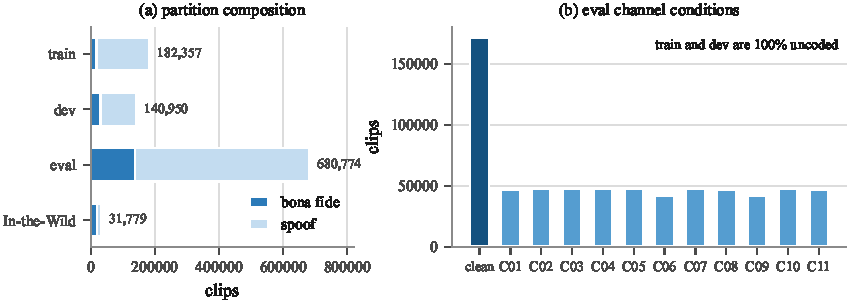
\includegraphics[width=\textwidth]{figures/fig10_dataset}
\caption{(a)~Partition composition. (b)~Evaluation-set channel conditions.
The selection split contains none of the eleven coded conditions the evaluation
set is judged on.}
\label{fig:dataset}
\end{figure}

% ------------------------------------------------------------------
\section{Systems}
\label{sec:systems}

\begin{figure}[t]
\centering
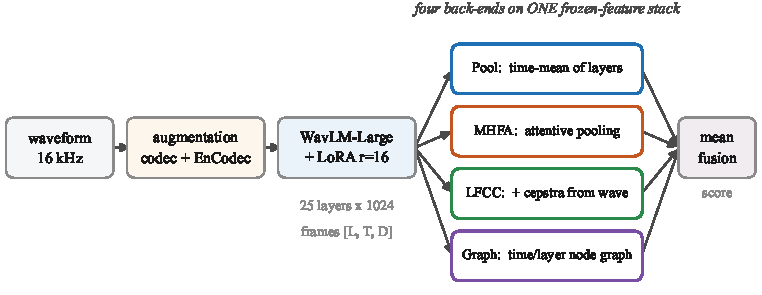
\includegraphics[width=\textwidth]{figures/fig1_architecture}
\caption{All four members share the waveform pipeline, the augmentation policy,
and the adapted WavLM-Large backbone, differing only in the back-end that maps
per-layer frames to a score.}
\label{fig:arch}
\end{figure}

Fig.~\ref{fig:arch} shows the common pipeline.  A waveform is augmented then
passed through WavLM-Large~\cite{wavlm} adapted with LoRA of rank~16 on the
attention projections~\cite{lora} (3.15M trainable parameters out of 315M
total).  The backbone emits 25 layer activations.  Training augmentation applies
one of eight simulated codecs with probability 0.5 and, with probability 0.3,
EnCodec~\cite{encodec} on the GPU---the neural codec corresponding to evaluation
conditions C04 and C07, which a CPU-bound DataLoader cannot apply.

\subsubsection{Pool.} (0.26M parameters.) Takes the time-\emph{mean} of each
layer, learns a softmax weighting over layers, and applies a two-layer MLP.
This is the conventional baseline design.

\subsubsection{MHFA.} (0.53M.) Keeps frames rather than pooling them first.
Following the speaker-verification architecture of Peng et al.~\cite{mhfa}, it
learns two \emph{separate} layer weightings---one producing keys, one
values---and pools over time by multi-head attention, so the layers that decide
\emph{where} to look need not be the layers carrying the evidence.

\subsubsection{LFCC.} (0.50M.) Adds a second \emph{representation}: 20
linear-frequency cepstral coefficients with first and second deltas, computed
from the waveform and aligned frame-for-frame with the backbone, then
concatenated before attentive pooling~\cite{attentive_pool}.  Part of its
evidence cannot correlate with anything the backbone encodes.

\subsubsection{Graph.} (0.30M.) Adds a second \emph{topology}: graph attention
over two node sets (time slots and backbone layers), reusing the graph attention
layer of AASIST~\cite{aasist}.  This is \emph{not} AASIST---there is no
heterogeneous cross-attention and no master node---and no result here should be
attributed to that architecture.

Members are combined by the unweighted mean of scores standardised on the
development \texttt{calib} split.  The combiner has no parameters fit on
evaluation data.

% ------------------------------------------------------------------
\section{Experimental Protocol}
\label{sec:protocol}

Models are selected on the development \texttt{select} split (attacks A09--A16),
scale statistics are fit on the speaker-disjoint \texttt{calib} half, and the
evaluation set is scored once.  Metrics are \eer{} and \mindcf{} under the
official ASVspoof~5 cost model (spoof prior $0.05$, $C_\text{miss}{=}1$,
$C_\text{fa}{=}10$)~\cite{asvspoof5,tdcf}, plus $\text{min}C_\text{llr}$.
Differences are tested with a paired bootstrap clustered on source utterance
(Section~\ref{sec:data}).

All members use seed 1337, batch size 32, eight epochs, head learning rate
$10^{-3}$ and backbone learning rate $10^{-5}$.  \textbf{Limitation stated up
front:} every member below is single-seed.  Earlier three-seed experiments on
this codebase gave a spread of 0.33~\eer{} points on frozen single models---larger
than the 0.10-point fusion gain we report.  Seed variance for systems in
Table~\ref{tab:members} is therefore unmeasured.

% ------------------------------------------------------------------
\section{Results}
\label{sec:results}

\subsection{Member Systems}

\begin{table}[t]
\centering
\small
\caption{The four members.  All share everything except the back-end.
Dev select is the mean \eer{} over the clean and codec development views.
$\rho_{\text{Pool}}$ is the Pearson correlation of evaluation scores with Pool.}
\label{tab:members}
\begin{tabular}{llrrrrrr}
\toprule
& & & \multicolumn{3}{c}{ASVspoof~5 eval} & \multicolumn{1}{c}{In-the-Wild} & \\
\cmidrule(lr){4-6}\cmidrule(lr){7-7}
Member & Back-end differs in & Dev sel. & \eer{} & \mindcf{} & min$C_\text{llr}$ & \eer{} & $\rho_{\text{Pool}}$ \\
\midrule
Pool  & ---             & \best{1.50} & 3.31 & 0.0942 & 0.1256 & 11.25 & --- \\
MHFA  & pooling         & 2.07 & 3.44 & 0.0957 & 0.1286 & \best{8.51} & 0.917 \\
LFCC  & representation  & 2.95 & \best{3.11} & \best{0.0845} & \best{0.1164} & 11.82 & 0.965 \\
Graph & topology        & 3.10 & 3.93 & 0.1091 & 0.1475 & 11.44 & 0.943 \\
\bottomrule
\end{tabular}
\end{table}

Table~\ref{tab:members} is the central table: almost every column disagrees with
every other.  Pool is the best member on development and only third on evaluation.
LFCC is the worst on development, the best on evaluation, and the worst again
in the wild.  MHFA goes from third in domain (3.44\%) to first out of domain
(8.51\%), a 24\% relative margin over the next system.

Fig.~\ref{fig:curves} shows these differences are not training artefacts.
Fig.~\ref{fig:det} gives the detection error trade-off curves; fused systems
dominate single members across the operating range.

\begin{figure}[t]
\centering
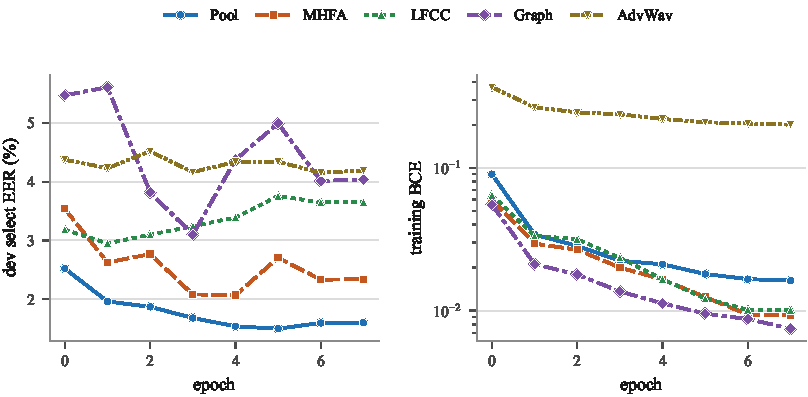
\includegraphics[width=\textwidth]{figures/fig2_training_curves}
\caption{Training behaviour.  Left: development \eer{}.  Right: training loss.
AdvWav (Section~\ref{sec:robust}) converges to roughly double the development
\eer{} of every other member.}
\label{fig:curves}
\end{figure}

\begin{figure}[t]
\centering
\begin{minipage}{0.48\textwidth}
  \centering
  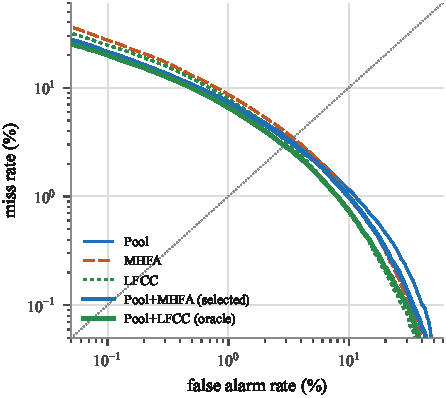
\includegraphics[width=\textwidth]{figures/fig3_det}
\end{minipage}\hfill
\begin{minipage}{0.48\textwidth}
  \centering
  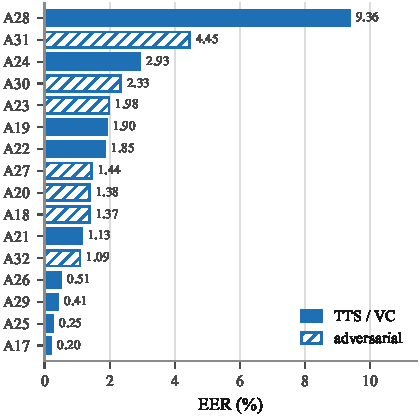
\includegraphics[width=\textwidth]{figures/fig5_per_attack}
\end{minipage}
\caption{Left: DET curves on the evaluation set; solid curves are fusions.
Right: per-attack \eer{} of the selected system.  The pooled number is dominated
by A28 (9.36\%); nine of sixteen attacks sit below 1.5\%.  Adversarial attacks
(hatched)~\cite{malafide,malacopula} are not the hard ones.}
\label{fig:det}
\end{figure}

\subsection{Conditions and Attacks}

Fig.~\ref{fig:codec} breaks down the evaluation set by channel.  The two neural
codecs, C04 and C07, are by a wide margin the hardest conditions for every
member---a direct consequence of their absence from uncoded training before we
added GPU-side EnCodec~\cite{encodec}.  Attack A28 alone accounts for 9.36\%
\eer{} while nine of sixteen attacks are under 1.5\%, so the pooled number is
largely a statement about one attack.  Attacker-adaptation conditions are
flat---AC1 3.29\%, AC2 3.14\%, AC3 3.19\%---so adaptation strength made no
measurable difference to us.

\begin{figure}[t]
\centering
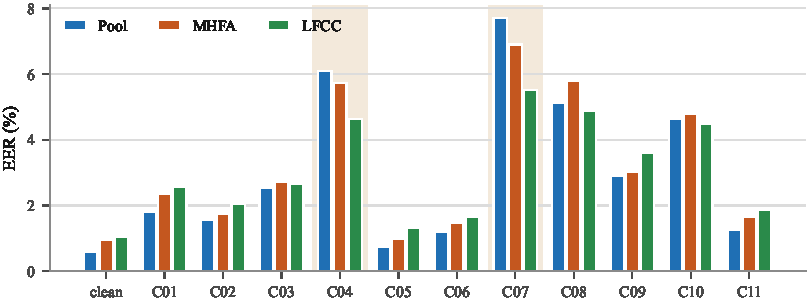
\includegraphics[width=\textwidth]{figures/fig4_per_codec}
\caption{Per-condition \eer{}.  The neural codecs C04 and C07 (shaded) are the
hardest conditions for every member; the development split contains neither.}
\label{fig:codec}
\end{figure}

\subsection{Effective System Count}
\label{sec:rank}

\begin{figure}[t]
\centering
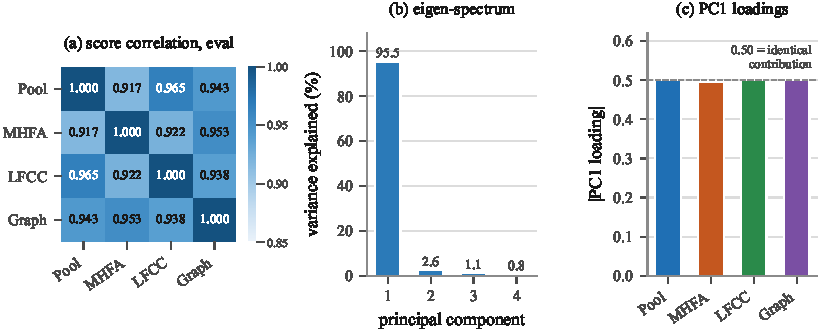
\includegraphics[width=\textwidth]{figures/fig6_spectrum}
\caption{(a)~Score correlation on the evaluation set.  (b)~Eigen-spectrum of
that matrix: PC1 explains 95.5\% of the variance.  (c)~PC1 loadings are within
0.006 of 0.50 on every member---the first component \emph{is} the unweighted mean.}
\label{fig:spectrum}
\end{figure}

We summarise a member set by the eigen-spectrum of its score correlation matrix,
reporting the participation ratio $(\sum_i \lambda_i)^2 / \sum_i \lambda_i^2$
and entropy rank $\exp(-\sum_i p_i \log p_i)$ with $p_i = \lambda_i / \sum_j \lambda_j$.
Both equal $1$ for identical systems and $M$ for orthogonal ones.

Fig.~\ref{fig:spectrum} gives the answer: \textbf{1.10 effective systems out of
four} (entropy rank 1.26), with PC1 explaining 95.5\% of the variance and loadings
$0.501, 0.496, 0.501, 0.502$.  On the out-of-domain set the figure is 1.15 of 4.
Changing pooling, representation, topology \emph{and} backbone shifts the effective
rank by only 0.1.

This reframes the fusion question.  The best two-member fusion improves on its best
member by 0.18~\eer{} points; a third member adds nothing.  The USTC-KXDIGIT system,
whose twelve systems across three back-end families gain 35\% relative from
fusion~\cite{ustc2024}, requires the kind of diversity our members lack.  The axis
that moved our correlation at all was the one that changed what the model
\emph{sees}, not how it is parameterised: replacing time-mean pooling with frame
attention moved correlation from 0.994 to 0.917.

\subsection{Selection Failure}
\label{sec:selection}

\begin{table}[t]
\centering
\small
\caption{Member subsets ranked by development \eer{}, top four of fifteen, plus
the best subset on evaluation.  The protocol selects row~1; the oracle row is
shown for comparison and is \emph{not} claimed as a result.}
\label{tab:selection}
\begin{tabular}{llrrrr}
\toprule
Rank & Subset & Dev sel. & eval \eer{} & eval \mindcf{} & ITW \eer{} \\
\midrule
\multicolumn{6}{l}{\emph{Selection on clean + codec ($\rho{=}+0.011$, $p{=}0.97$)}}\\
1 & Pool + MHFA          & \best{1.46} & 3.21 & 0.0905 & 9.04 \\
2 & Pool                 & 1.47 & 3.31 & 0.0942 & 11.25 \\
3 & Pool + MHFA + Graph  & 1.67 & 3.20 & 0.0903 & 8.80 \\
4 & Pool + MHFA + LFCC   & 1.72 & 2.94 & 0.0827 & 9.04 \\
7 & \emph{Pool + LFCC} (oracle) & 1.83 & \emph{2.93} & \emph{0.0819} & 9.19 \\
\midrule
\multicolumn{6}{l}{\emph{Selection with neural-codec view added ($\rho{=}+0.236$, $p{=}0.40$)}}\\
1 & Pool + MHFA          & \best{2.79} & 3.21 & 0.0905 & 9.04 \\
2 & Pool + MHFA + LFCC   & 2.90 & 2.94 & 0.0827 & 9.04 \\
6 & \emph{Pool + LFCC} (oracle) & 3.01 & \emph{2.93} & \emph{0.0819} & 9.19 \\
\bottomrule
\end{tabular}
\end{table}

\begin{figure}[t]
\centering
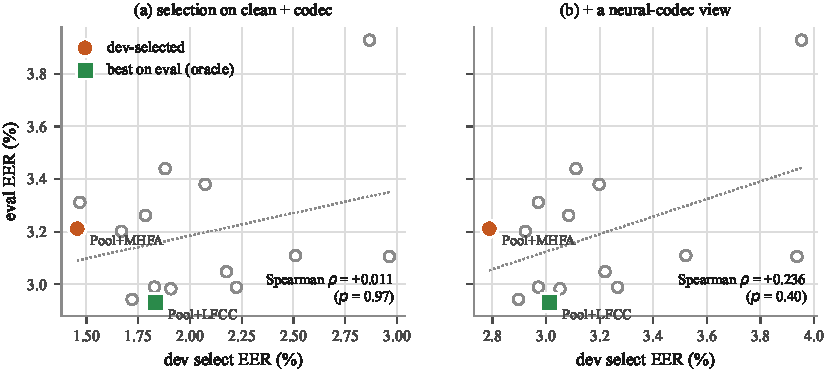
\includegraphics[width=\textwidth]{figures/fig7_selection}
\caption{Development \eer{} against evaluation \eer{} for all 15 member subsets.
Adding a neural-codec view improves ordering---the three-member system climbs
from rank~4 to rank~2---but does not make selection predictive.}
\label{fig:selection}
\end{figure}

Over all 15 subsets, $\rho{=}+0.011$ ($p{=}0.97$): the development split carries
no information about evaluation ordering (Fig.~\ref{fig:selection}).  Since the
evaluation set's discriminating conditions are real codecs absent from development,
we added a neural-codec development view.  This helps ($\rho$ rises to $+0.236$,
the three-member system climbs from rank~4 to rank~2), but at $p{=}0.40$ it is
still indistinguishable from zero.

\textbf{We report the protocol-selected result and the oracle bound, and take the
0.28-point gap between them as a measurement of the selection set.}  Our selected
system is Pool\,+\,MHFA at \textbf{3.21\% \eer{} / 0.0905 \mindcf{}}.  The oracle
is Pool\,+\,LFCC at \emph{2.93\% / 0.0819}, ranked seventh of fifteen by our
protocol.

\subsection{Domain Transfer}

\begin{figure}[t]
\centering
\begin{minipage}{0.48\textwidth}
  \centering
  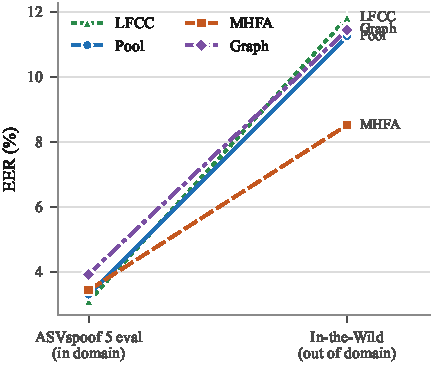
\includegraphics[width=\textwidth]{figures/fig8_transfer}
\end{minipage}\hfill
\begin{minipage}{0.48\textwidth}
  \centering
  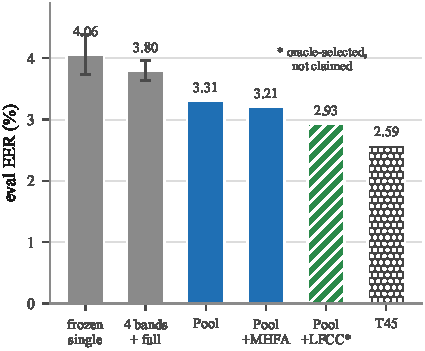
\includegraphics[width=\textwidth]{figures/fig9_progress}
\end{minipage}
\caption{Left: all systems degrade $2.5$--$3.8\times$ out of domain and the
ordering inverts.  Right: progression of this work; bars with error bars are
three-seed means; the hatched bar is oracle-selected.}
\label{fig:transfer}
\end{figure}

Fig.~\ref{fig:transfer} (left) shows the $2.5$--$3.8\times$ degradation found by
M\"{u}ller et al.~\cite{intothewild} more broadly.  What is not routine is the
inversion: LFCC, our best in-domain member at 3.11\%, is our worst in the wild at
11.82\%, while MHFA goes from third (3.44\%) to first (8.51\%).

A plausible reading is that cepstral features partly capture recording-condition
statistics, which do not transfer from a curated corpus to found audio, whereas
frame-level attention learns something less corpus-specific.  We offer this as a
hypothesis; our experiments establish the inversion, not its cause.  The practical
implication is that pursuing the final 0.6~\eer{} points in domain would mean
preferring the member that transfers worst.

% ------------------------------------------------------------------
\section{Adversarial Robustness}
\label{sec:robust}

\begin{table}[t]
\centering
\small
\caption{Attack success at a 0.1\% false-alarm operating point, 20-step PGD
under an SNR-constrained $L_2$ budget~\cite{madry2018}.  Realised SNR is
reported, not assumed.  Generated from attack logs; the table cannot drift from
measurements.  Four routes are closed outright; waveform adversarial training is
the only one that moves white-box success off 1.000.}
\label{tab:robust}
% generated by paper/robustness_table.py -- do not edit by hand
\begin{tabular}{llrrr}
\toprule
Defence & Attack & Clean \eer{} & 30\,dB & 20\,dB \\
\midrule
single model & white-box PGD & 4.78 & 1.000 & 1.000 \\
single model & SPSA & 4.78 & --- & 0.011 \\
four layer bands & white-box PGD & 4.78 & 1.000 & 1.000 \\
four layer bands & transfer PGD & 4.78 & 1.000 & 1.000 \\
four layer bands & SPSA & 4.78 & --- & 0.014 \\
WavLM, surrogate XLS-R & white-box PGD & 4.78 & 1.000 & 1.000 \\
WavLM, surrogate XLS-R & transfer PGD & 4.78 & 0.892 & 0.995 \\
XLS-R, surrogate WavLM & white-box PGD & 9.21 & 1.000 & 1.000 \\
XLS-R, surrogate WavLM & transfer PGD & 9.21 & 0.832 & 0.984 \\
feature-space adv.\ training & white-box PGD & 13.95 & 0.993 & 1.000 \\
feature-space adv.\ training & transfer PGD & 13.95 & 0.776 & 0.977 \\
\textbf{waveform adv.\ training} & white-box PGD & 7.07 & 0.953 & 0.967 \\
\textbf{waveform adv.\ training} & transfer PGD & 7.07 & 0.739 & 0.951 \\
its control (Pool) & white-box PGD & 4.17 & 1.000 & 1.000 \\
its control (Pool) & transfer PGD & 4.17 & 1.000 & 1.000 \\
\bottomrule
\end{tabular}

\end{table}

Table~\ref{tab:robust} summarises the robustness measurements.
We use PGD~\cite{madry2018}, a projected gradient descent attack under an
SNR-constrained $L_2$ budget; a query-limited SPSA black-box attacker with 320
queries per clip; and white-box / transfer variants.  A gradient-bearing attacker
succeeds on essentially every clip at 30\,dB SNR against four of the five
defences: a single model, a four-member band ensemble, each of two SSL backbones
used as the other's surrogate, and feature-space adversarial
training---which additionally destroyed clean accuracy to 13.95\% \eer{}.
A black-box attacker with 320 queries succeeds on about 1\%.

\textbf{Waveform adversarial training is the one route that moves.}
Hardening the path the attacker actually takes---half of each batch replaced by
30\,dB PGD examples crafted through the backbone---drops white-box success from
1.000 to 0.953 at 30\,dB, and transfer success from 1.000 to 0.739.  Its matched
control, trained without the adversarial half, sits at 1.000 on every row, so the
drop is the defence.

\textbf{The price is severe.}  Clean evaluation \eer{} rises from 3.31\% to
7.09\%, a paired difference of $+0.0378$ ($95\%$ CI $[+0.0372,\,+0.0384]$ over
680{,}774 clips).  Codec conditions take the worst damage (C07 11.06\%, C08
10.08\%).  Buying a 4.7-point reduction in white-box success for 3.78 \eer{}
points of clean accuracy is not a trade any deployed system would take.

Our contribution here is therefore a measurement rather than a method: under this
threat model the SSL detectors in this paper are not defensible at usable accuracy,
and the one defence that addresses the right surface shifts the frontier without
crossing it.  The feature-space row is a corrected experiment: it was defending
the wrong path~\cite{madry2018}, and correcting the mismatch recovered 6.9 \eer{}
points of clean accuracy while also being the change that moved white-box success
at all.

% ------------------------------------------------------------------
\section{Limitations}
\label{sec:limit}

\textbf{Single seed.}  Every system in Table~\ref{tab:members} is one seed.
Earlier three-seed experiments gave a 0.33~\eer{} point spread on frozen single
models, larger than the 0.10-point fusion gain.  The fusion gain is not established
against seed variance.

\textbf{One corpus.}  We train on ASVspoof~5 alone.  USTC-KXDIGIT~\cite{ustc2024}
trains on four corpora.  We cannot separate a weaker architecture from narrower
supervision.

\textbf{Clustered intervals matter.}  Clip-level bootstrap intervals on this
corpus are about $2\times$ too narrow.  Our conclusions survive the correction
because differences are many standard errors wide, but intervals reported elsewhere
on this corpus may not.

\textbf{One out-of-domain set.}  In-the-Wild has its own biases: public figures,
internet audio, an inverted class prior.  One such set measures a gap; it does not
characterise generalisation.

\textbf{The graph member is not AASIST} and results should not be cited as
evidence about AASIST~\cite{aasist}.

% ------------------------------------------------------------------
\section{Conclusion}
\label{sec:conclusion}

Four detectors differing in pooling, representation, topology, and backbone amount
to 1.10 independent systems.  Architectural variety is not the same as error
diversity; only a change in what the model \emph{sees} moved the correlation.
The development split of the corpus everyone uses cannot rank these systems,
costing 0.28~\eer{} points against its own oracle; and in-domain ranking inverts
out of domain, so the best leaderboard member transfers worst.

Our selected system reaches \textbf{3.21\% \eer{} / 0.0905 \mindcf{}}, ahead of
SZU-AFS at 4.04\% / 0.115~\cite{szuafs} and short of the twelve-system winner at
2.59\% / 0.0750~\cite{ustc2024}.  The more useful contribution is the measurement
around that number: a reproducible way to quantify how many systems an ensemble
really contains, and evidence that the standard selection procedure on this
benchmark does not work.

\subsubsection*{Reproducibility.}
Figures are generated by \texttt{paper/make\_figures.py} from a single JSON of
measured values, so no number in the text can disagree with a figure.  Every
experiment, including failures and incorrect predictions, is recorded in
\texttt{docs/experiment\_log.md}.

% ------------------------------------------------------------------
\bibliographystyle{splncs04}
\bibliography{refs}

\end{document}
